\documentclass[10pt]{beamer}

\usetheme[progressbar=frametitle]{metropolis}
\usepackage{appendixnumberbeamer}

\usepackage[autoplay]{animate}
\usepackage{graphicx}
\usepackage{subcaption}

\usepackage{booktabs}
\usepackage[scale=2]{ccicons}

%\usepackage{pgfplots}
%\usepgfplotslibrary{dateplot}

\usepackage{xspace}

\setbeamercolor{normal text}{bg=white}
\newcommand{\themename}{\textbf{\textsc{metropolis}}\xspace}

\title{Examining Hausdorff dimension and Scaling behaviour with Worm algorithm}
%\subtitle{A modern beamer theme}
\date{\today}
\date{}
\author{Simon Rydell}
\institute{Royal Institute of Technology, Stockholm}
% \titlegraphic{\hfill\includegraphics[height=1.5cm]{logo.pdf}}

\begin{document}

\maketitle

\begin{frame}{Table of contents}
  \setbeamertemplate{section in toc}[sections numbered]
  \tableofcontents[hideallsubsections]
\end{frame}

\section{Fractals}

\begin{frame}{Scaling Mass}
    hi
\end{frame}

\begin{frame}{A Measure of Roughness}
    hi
\end{frame}

\begin{frame}{Box Counting Method}
    hi
\end{frame}

\begin{frame}{Hausdorff Dimension}
    hi
\end{frame}

\section{Algorithms Used For Generating Graph Patterns}

\begin{frame}{Worm Algorithm}
    Idea is to sample non-zero contributions of the partition function at $T = T_c$. Express them in a way as to form `loops'.
\end{frame}

\begin{frame}{Hoshen Kopelman Labeling and Graph Dividing}
    Idea is to sample non-zero contributions of the partition function at $T = T_c$. Express them in a way as to form `loops'.
\end{frame}

\section{Ising Model}

\begin{frame}{Ising Loop Expansion}
    \begin{equation*}
        Z &\propto  \sum_{\{S\}} \left ( 1 + \tanh(K) \sum_{l = 1} S_i S_j + \tanh^2(K) \sum_{l = 2} (S_i S_j)(S_{i'} S_{j'}) + \ldots \right)
    \end{equation*}
% The idea is to expand the ising partition to these sums over pairs of spins. The sum subscript represent the contiguous length of this link. 
\end{frame}

\begin{frame}{Ising Loop Expansion}
\begin{figure}[h!]
    \begin{subfigure}{.4\linewidth}
        \centering
        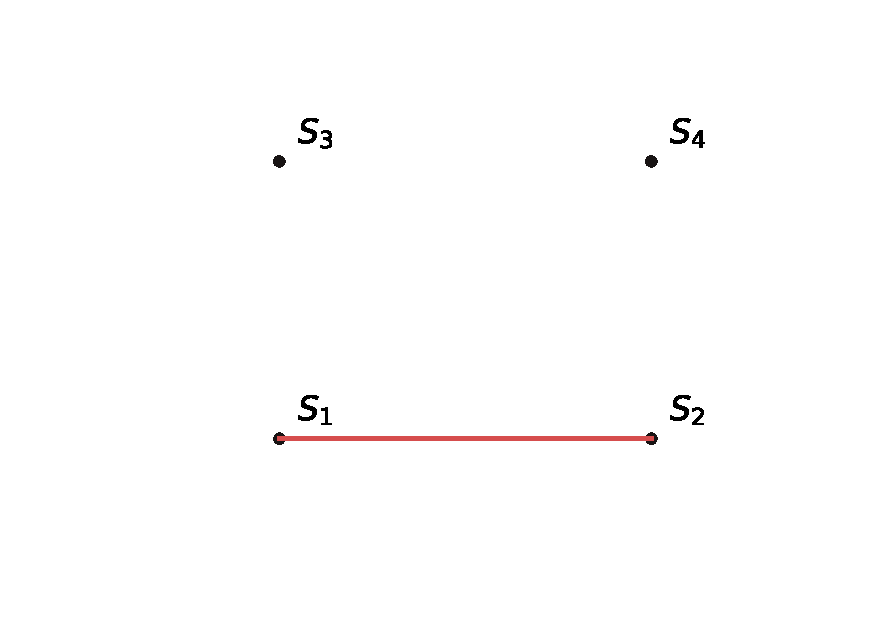
\includegraphics[width=\textwidth]{figures/ising_loop_one_link.pdf}
        \caption{$(S_1 S_2), \ L = 1$}
    \end{subfigure}%
    \begin{subfigure}{.4\linewidth}
        \centering
        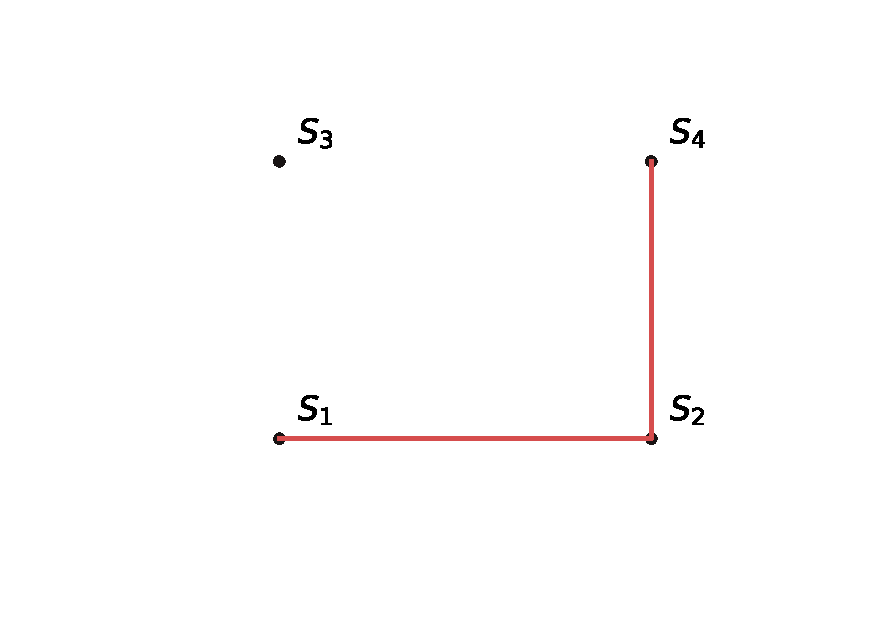
\includegraphics[width=\textwidth]{figures/ising_loop_two_link.pdf}
        \caption{$(S_1 S_2)(S_2 S_4), \ L = 2$}
    \end{subfigure}\\[1ex]
    \begin{subfigure}{.8\linewidth}
        \centering
        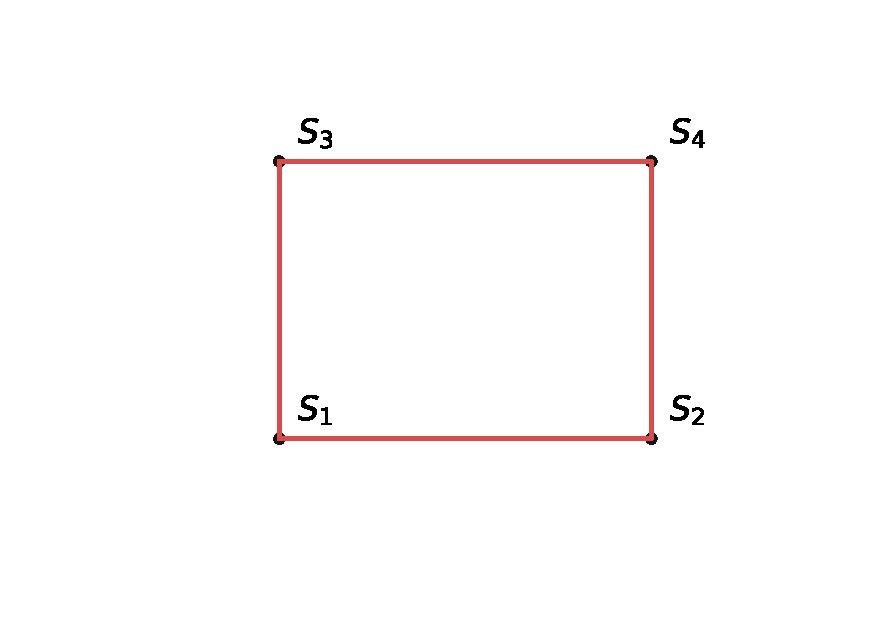
\includegraphics[width=.5\textwidth]{figures/ising_loop_four_link.pdf}
        \caption{$(S_1 S_2)(S_2 S_4)(S_4 S_3)(S_3 S_1), \ L = 4$}
    \end{subfigure}
\end{figure}
% Here we can see the link structure in between sites. Since the partition function includes a sum over all states of each individual spin, in this case +1 and -1, only the terms with a full loop will survive, since these only have terms such as $S_i^2$.
\end{frame}


\begin{frame}{Box Dimension}
    \begin{figure}[h!]
        \centering
            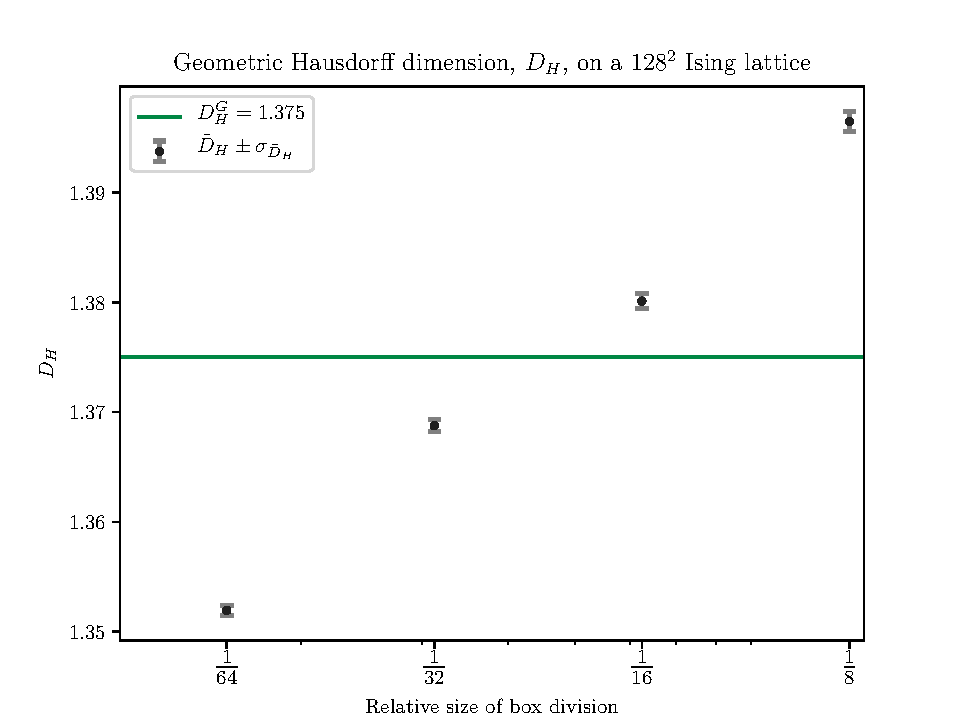
\includegraphics[width=0.8\textwidth]{figures/box_dim_128x128Ising.pdf}
    \end{figure}
% Given enough sampling, a physical system will emerge. This can then be divided as per the discussed box counting method. The result is here compared to the theoretical one given by Loewner expansion.
\end{frame}

\begin{frame}{Scaling Dimension}
    \begin{figure}[h!]
        \centering
            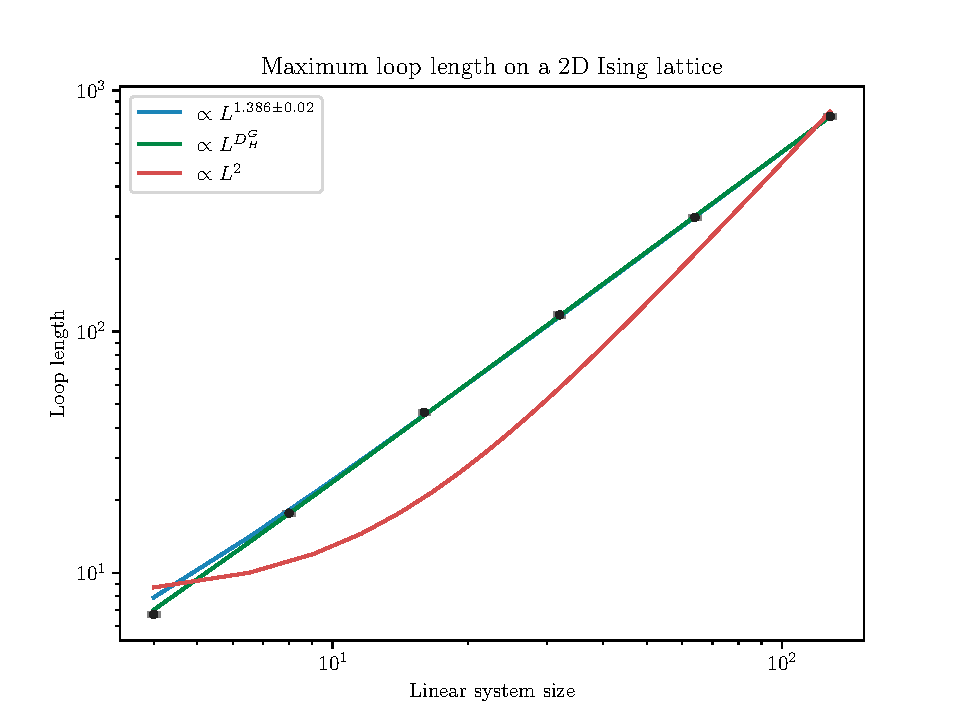
\includegraphics[width=0.8\textwidth]{figures/maximum_loop_length_for_2D_Ising.pdf}
    \end{figure}
% If we instead use the scaling method, the result is this. The theoretical value can almost be seen under the line fit. The red line here is just for comparison.
\end{frame}

\begin{frame}{Comparison of Dimensions $2D$ Ising}
    \begin{figure}[h!]
        \centering
            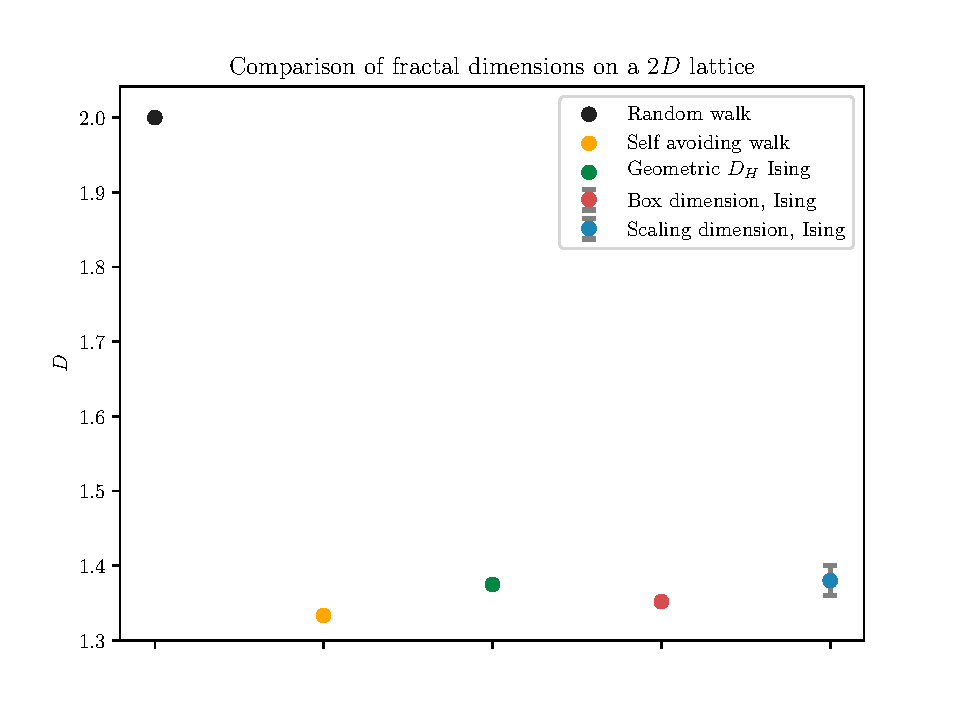
\includegraphics[width=0.8\textwidth]{figures/dimenson_comparison.pdf}
% Peculiar enough, the clusters has almost the same hausdorff dimension as a self avoiding walk, shown here in yellow. This suggest some similarities between the structure of the SAW and the ising clusters
    \end{figure}
\end{frame}

\begin{frame}{Largest Ising Loop on a $128^2$ Lattice}
    \begin{figure}[h!]
        \centering
            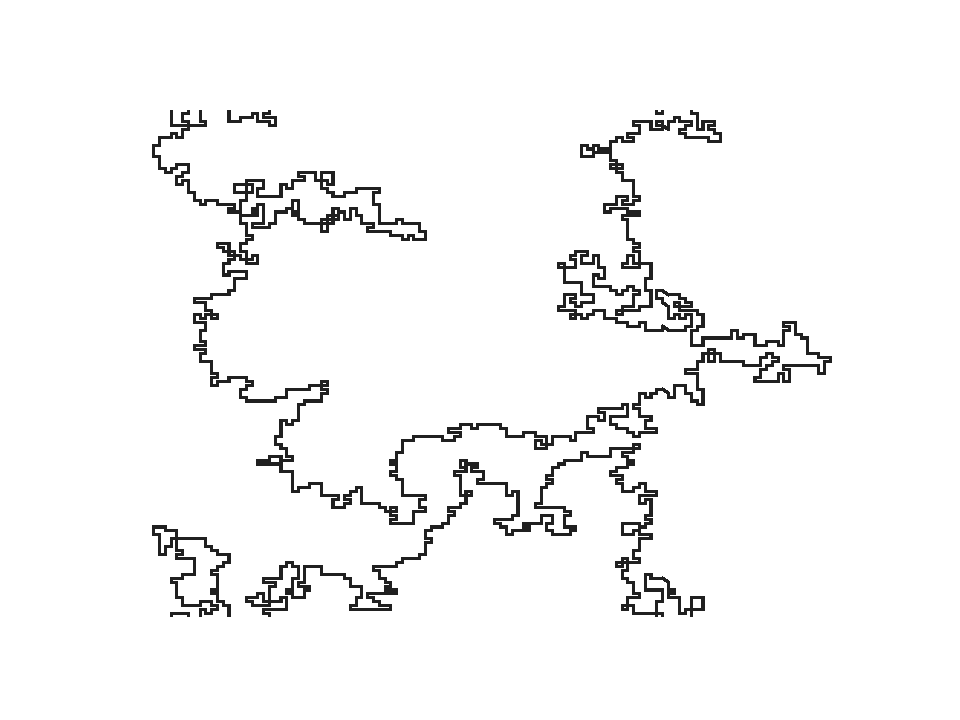
\includegraphics[width=0.8\textwidth]{figures/largest_cluster_testing_nolattice.pdf}
    \end{figure}
% If we further examine a cluster on a 128^3 ising lattice we can see the familiar `swollen' structure in the loop. The only visible difference here is that `twisted loops' are allowed as it doesn't cost any energy to create them in the worm algorithm.
% To further get intuition about how this process is done, I created a small animation of a 2D Ising lattice. From the point where some clusters have formed, we identify the largest cluster with the Hoshen Kopelman algorithm and the lattice is divided into smaller and smaller boxes.
\end{frame}

\begin{frame}{$2D$ Ising Animation}
    % TODO: Uncomment
    %  \animategraphics[width=\linewidth,loop]{10}{figures/2dising_animation}{}{}
\end{frame}

\section{XY Model}
% Rotors... Loop Expansion. Adds complexity as a direction and weight. Use Villain approximation $\Rightarrow$ Displaces $T_c$ $\Rightarrow$ Use winding number to `find' $T_c$.

\begin{frame}{XY Loop Expansion}
    \begin{align*}
        H &= - J \sum_{\langle ij \rangle} \cos(\theta_i - \theta_j) \\
        Z &= \prod_i \int \frac{\mathrm d \theta_i}{2 \pi} \prod_{\langle ij \rangle} e^{K  \cos(\theta_i - \theta_j)}
% The XY model allows spin to rotate around some axis in a plane. Giving a Hamiltonian as a function of the difference in angle in this plane. 
% Therefore we get the 2 pi symmetric partition function, that can be fourier transformed as
    \end{align*}
\end{frame}

\begin{frame}{XY Loop Expansion}
    \begin{align*}
        Z &\sim \int \frac{\mathrm d \theta_i}{2 \pi} e^{i \sum_{\langle ij \rangle} j_{\langle ij \rangle} (\theta_i - \theta_j)} \\
% Where lower case j here is the fourier coefficients summed over the nearest neighbours. Expanding this integral shows
    \end{align*}
\end{frame}

\begin{frame}{XY Loop Expansion}
    \begin{align*}
        Z &\sim \int \frac{\mathrm d \theta_i}{2 \pi} e^{i \sum_{\langle ij \rangle} j_{\langle ij \rangle} (\theta_i - \theta_j)} \\
        & \sim \delta_{0, \sum_{\langle ij \rangle} j_{\langle ij \rangle}}
% that the sum of the links from each site to its neighbours must be zero. We can convince ourselves that this in turn means that the links together will form loops.
% This does add a bit of complexity compared to the Ising loop expansion. Here each link can have either positive or negative values, so we interpret this as direction. So instead of connecting site a and b, we connect site a to b with some weight w, giving something like this...
    \end{align*}
\end{frame}

\begin{frame}{XY Loop expansion}
    \begin{figure}[h!]
        \centering
            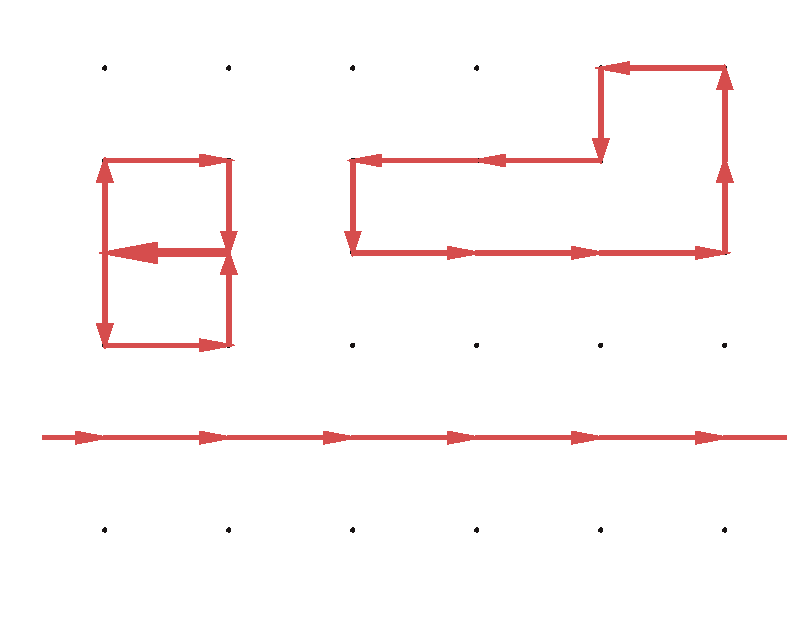
\includegraphics[width=0.8\textwidth]{figures/percolatingFlux.pdf}
    \end{figure}
% To simplify the acceptance probability I used the Villain approximation where the energy is simply the sum of these fourier coefficients squared.
\end{frame}

\begin{frame}{Villain Approximation}
    \begin{equation*}
        E = \frac{1}{2} \sum_i j_i^2
    \end{equation*}
% In this approximation, the notion of temperature is exchanged for one over temperature, leading to a shift in the critical temperature. One way to find the new Tc is to examine the superfluid density of the system, and notice that it is proportional to an easily measurable quantity called the winding number
\end{frame}


\begin{frame}{Winding Number}
    \begin{equation*}
        \rho_s = L^{2 - d} T \langle W_\mu^2 \rangle 
    \end{equation*}
% Where rho_s is the superfluid density and W_mu is the winding number in the mu direction. Intuitively, this says something about how many times the current percolates in the mu direction.
% We can then plot the winding number for a range of temperatures and system sizes to look for an intersection where the superfluid density goes to zero.
\end{frame}

\begin{frame}{Winding Number}
    \begin{figure}[h!]
        \centering
            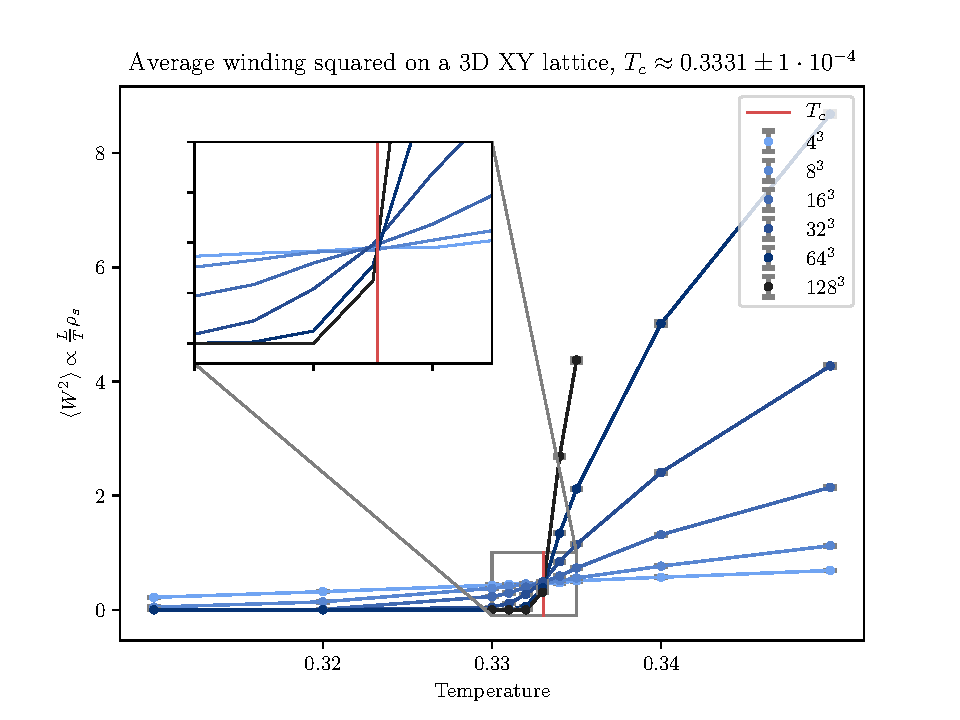
\includegraphics[width=0.8\textwidth]{figures/winding_number_Tc_zoomed.pdf}
    \end{figure}
% which is done here. The darker the blue, the larger the system is, and the intersection showed in red is taken as the weighted average of the intersections of all system sizes.
% Now that the critical temperature is known, the fractal dimension of the clusters can be examined.
\end{frame}

\begin{frame}{$3D$ XY Model Hausdorff Dimension}
    \begin{enumerate}[$\bullet$]
        \item Hove, Mo and Sudbo: $D_H = 2.287 \pm 4 \cdot 10^{-3}$
        \item Prokof'ev and Svistunov Comment: $D_H = 1.7655 \pm 2 \cdot 10^{-3}$
    \end{enumerate}
% In the year 2000 Hove, Mo and Sudbo published 
\end{frame}

\begin{frame}{Box Counting Method $3D$ XY}
    \begin{figure}[h!]
        \centering
            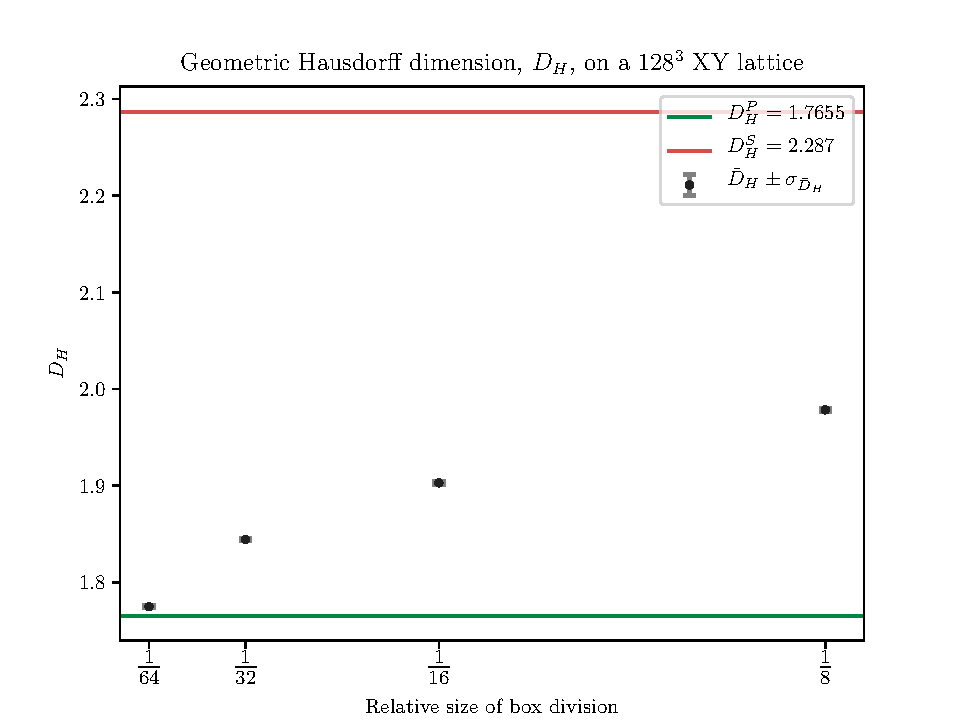
\includegraphics[width=0.8\textwidth]{figures/box_dimension_xy_128x3.pdf}
    %    \caption{}
    %    \label{fig:}
    \end{figure}
\end{frame}

\begin{frame}{Comparison of Dimensions $3D$ XY}
    \begin{figure}[h!]
        \centering
            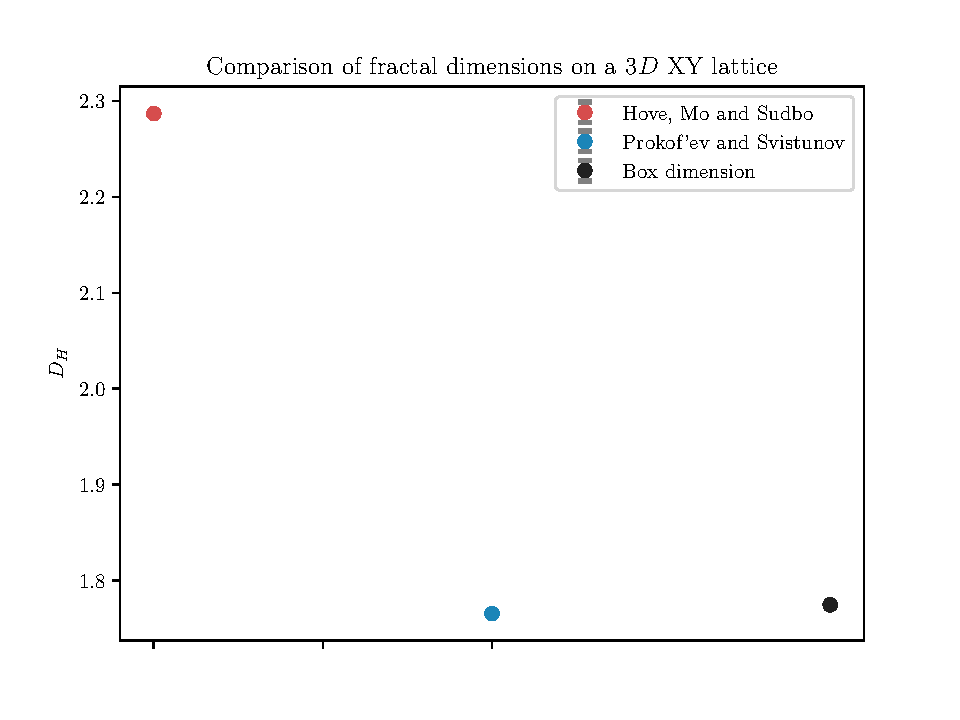
\includegraphics[width=0.8\textwidth]{figures/dimenson_comparison_XY.pdf}
    %    \caption{}
    %    \label{fig:}
    \end{figure}
\end{frame}


\begin{frame}{$3D$ XY Animation}
%  \animategraphics[width=\linewidth,loop]{10}{figures/3dxy_animation}{}{}
\end{frame}

\begin{frame}{Summary}
    \begin{table}
        \parbox{.45\linewidth}{
            \centering
            \begin{tabular}{l|l}
                               & $D_H$          \\ \hline
                Box            & $1.35193(5)$   \\ \hline
                Scaling        & $1.38(2)$      \\ \hline
                $D_H^G$        & $1.375$        \\ \hline
                SAW            & $1.33$         \\ \hline
                Random Walk    & $2$                          
            \end{tabular}
            \caption{$2D$ Ising}
        }
        \hfill
        \parbox{.45\linewidth}{
            \centering
            \begin{tabular}{l|l}
                            & $D_H$           \\ \hline
                Box         & $1.77468(4)$    \\ \hline
                Prokof'ev   & $1.765(2)$      \\ \hline
                Sudbo       & $2.287(2)$  
            \end{tabular}
            \caption{$3D$ XY}
        }
    \end{table}
\end{frame}

\appendix
% --------------- Backup slides ---------------

% --------------- Ising ---------------
\begin{frame}[fragile]{Backup slides: Box Dimension $64^2$ Ising}
    \begin{figure}[h!]
        \centering
            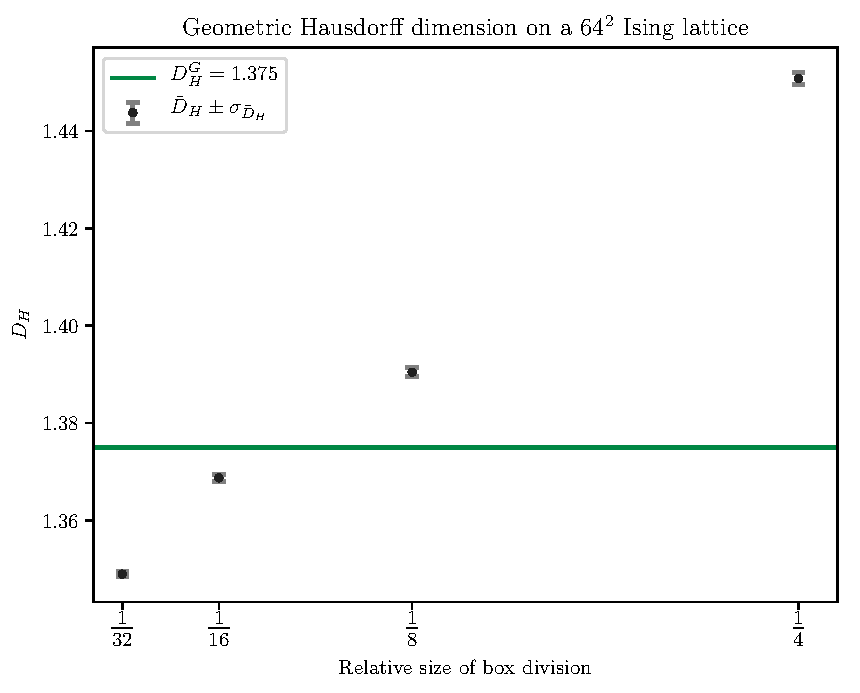
\includegraphics[width=0.8\textwidth]{figures/box_dim_64x64Ising.pdf}
    %    \caption{}
    %    \label{fig:}
    \end{figure}
\end{frame}

\begin{frame}[fragile]{Backup slides: Susceptibility $2D$ Ising}
    \begin{figure}[h!]
        \centering
            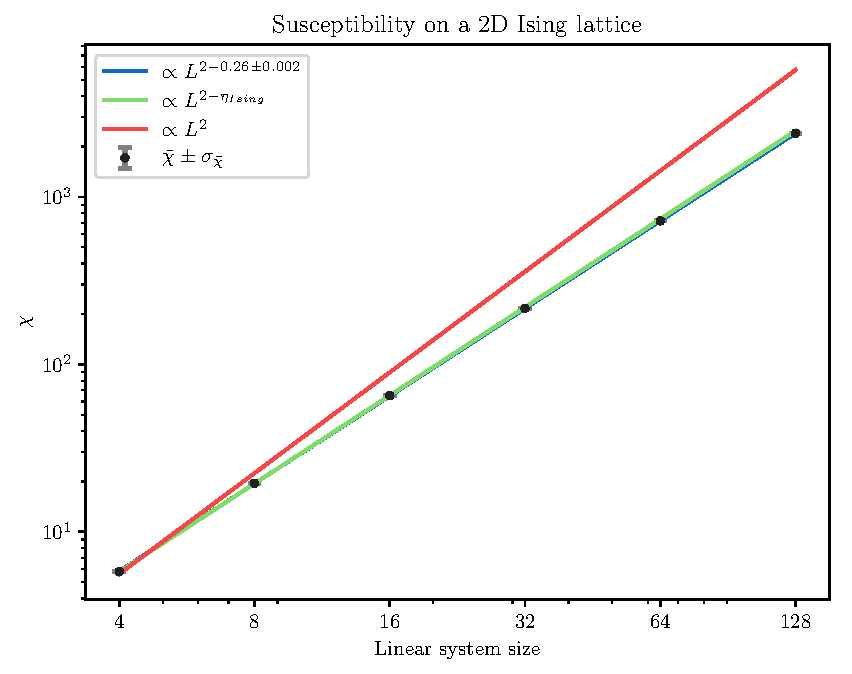
\includegraphics[width=0.8\textwidth]{figures/susceptibility128x128Ising.pdf}
    %    \caption{}
    %    \label{fig:}
    \end{figure}
\end{frame}

% --------------- Graph Dividing ---------------

\begin{frame}[fragile]{Backup slides: Graph Dividing Algorithm}
    \begin{figure}[h!]
        \centering
            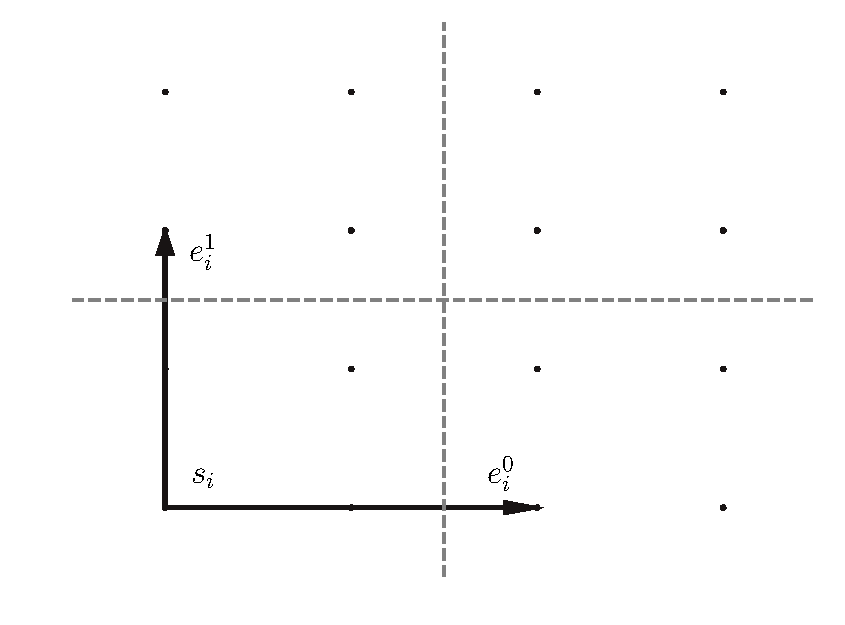
\includegraphics[width=0.8\textwidth]{figures/graphDividing.pdf}
    %    \caption{}
    %    \label{fig:}
    \end{figure}
\end{frame}

\begin{frame}[fragile]{Backup slides: Graph Dividing Algorithm}
    \begin{figure}[h!]
        \centering
            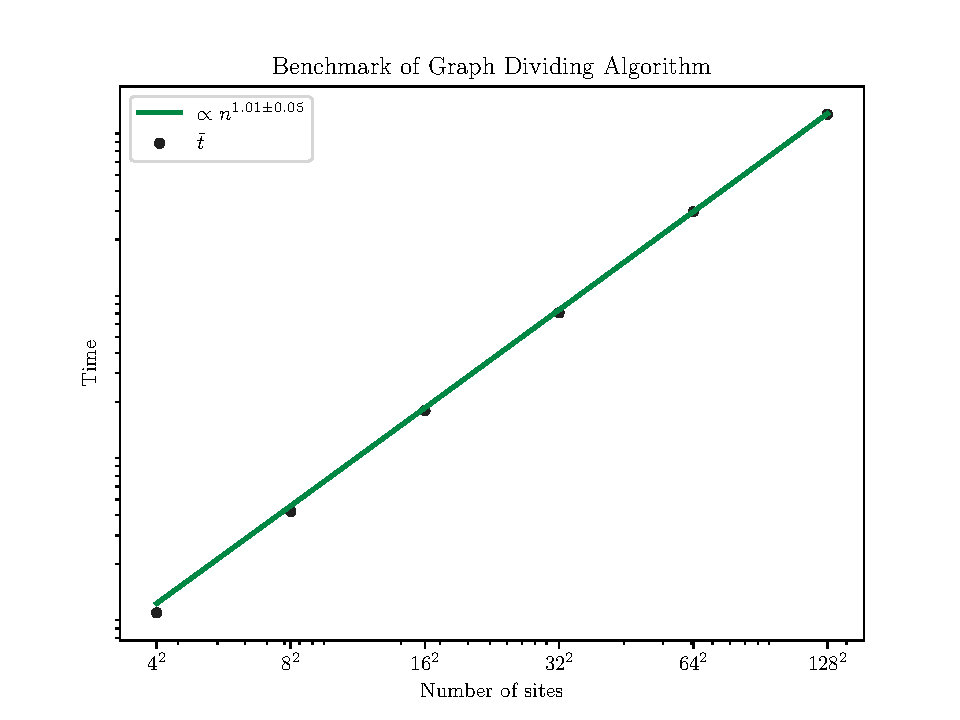
\includegraphics[width=0.8\textwidth]{figures/bench_graph_div.pdf}
    %    \caption{}
    %    \label{fig:}
    \end{figure}
\end{frame}


\end{document}